%%%%%%%%%%%%%%%%%%%%%%%%%%%%%%%%%%%%%%%%%%%%%%%%%%%%%%%%%%%%%%%%%%%%%%%%%%
%%%%%%%%%%%%   CAPTER 3   %%%%%%%%%%%%%%%%%%%%%%%%%%%%%%%%%%%%%%%%%%%%%%%%
%%%%%%%%%%%%%%%%%%%%%%%%%%%%%%%%%%%%%%%%%%%%%%%%%%%%%%%%%%%%%%%%%%%%%%%%%%
\chapter{Baseline Analysis}
\label{chap:existing_analysis}
This chapter explains the baseline analysis carried out by Airbus DS\cite{fcas}. An airborne Radar processor should be capable of processing both the Air to Air Mode data as well as Air to Ground Mode data. The scope of this thesis is limited to A/A Mode processing. Implementation is not done for the baseline analysis. So, it only estimates the approximate processing latency, CPU utilization and memory utilization with reference to the functional block execution cycle listed in the Tables \ref{tbl:aa_exe} and \ref{tbl:aa_exe}. The baseline analysis configures scheduling schemes in accordance to Space Partition and Time Partition.
\vspace*{2mm} \\
\noindent
\textbf{Time Partitioning:}\\
One iMX6Quad CPU is time sliced to run A/A mode and A/G mode alternatively. The timeframe between two subsequent A/A mode execution is called major time frame. Memory and cache are also partitioned for each mode. Intra-partition communication can be done by buffers, semaphores and/or events. When the time slice is completed for Air to Air mode, context switch happens to store the details of A/A Mode and load the details of A/G Mode, afterwards the A/G mode begins execution. Violation of timing behaviour triggers an exception. 
\vspace*{2mm} \\
\noindent
\textbf{Space Partitioning:} \\
A/A mode processing and A/G mode processing are done in separate physical entities. It is the simplest configuration for dedicated data processing. Failure of one of the systems will not affect the other as they are independent. It is assumed that SDRAM and L2 cache are partitioned for 4 cores to improve determinism. Each core has pre-defined accessible address space in Memory and L2 cache. 

%%%%%%%%%%%%%%%%%%%%%%%%%%%%%%%%%%%%%
%%%%%%%%%%%%%%%%%%%%%%%%%%%%%%%%%%%%%
%%%%%%%%%%%%   SECTION   %%%%%%%%%%%%
%%%%%%%%%%%%%%%%%%%%%%%%%%%%%%%%%%%%%
%%%%%%%%%%%%%%%%%%%%%%%%%%%%%%%%%%%%%
\section{Scheme 1 - Space Partitioning}
\label{sec:scheme_1}
A Radar echo received by the Radar antenna is distinguished as A/A mode or A/G mode by the iCON1 module. 
\begin{figure}[h!]
	\centering
	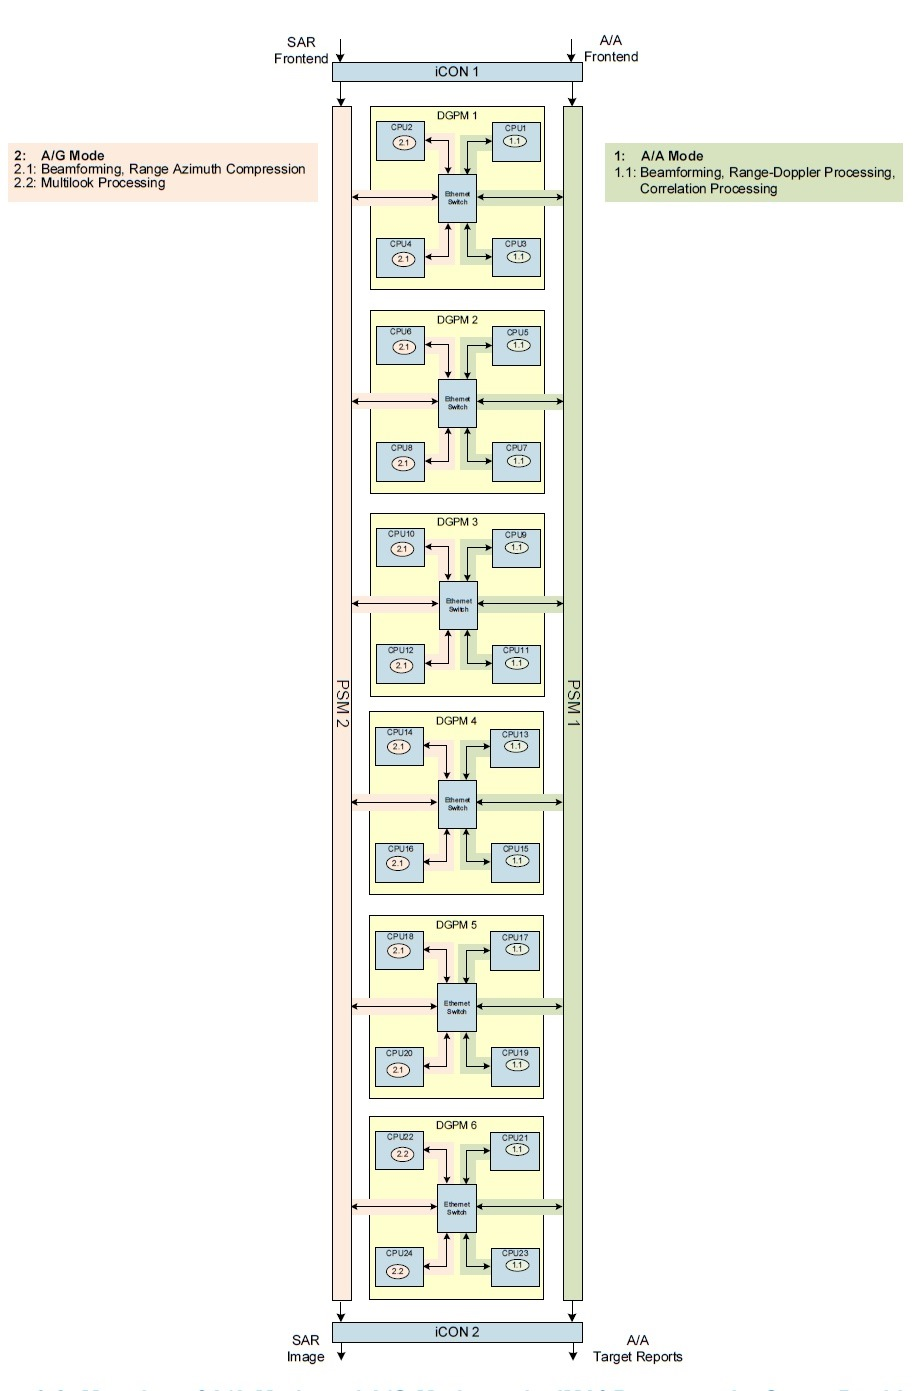
\includegraphics[width=160mm, height=220mm]{figures/scheme1}
	\caption{ Scheduling Scheme}
	\label{fig:existing_analysis:scheme1}
\end{figure}
\FloatBarrier
A/A mode data are redirected to PSM1 and A/G mode data are sent to PSM2. Figure \ref{fig:existing_analysis:scheme1} shows the mapping of A/A Mode and A/G Mode to the IMA processor architecture. The two odd numbered CPUs(CPU1 and CPU3 of DGPM1) of a  DGPM are allocated to the processing of the A/A mode. The two even numbered CPUs(CPU2 and CPU4 of DGPM1)  of a DPGM are allocated to the processing of the A/G mode. Each CPU with it's 4 cores is completely used for either A/A Mode or A/G mode processing.


\begin{tabular}{rl}
	Number of DGPMs: & 6 \\
	Number of CPUs: & 6 x 4 = 24 \\
	CPUs for A/A Mode: & 12 \\
	CPUs for A/G Mode: & 12 \\
\end{tabular}

\noindent
DGPM sends the processed data to iCON2 via respective PSM. iCON2 redirects A/A data to the Tracking processor and A/G data to the Display processor. The SDRAM is assumed to be partitioned for all the four cores, where every core has its buffer memory intended to transfer data between the cores and storage memory to store the data for Radar processing.

%%%%%%%%%%%%%%%%%%%%%%%%%
%%%%%   SUB-SECTION   %%%
%%%%%%%%%%%%%%%%%%%%%%%%%
%%%%%%%%%%%%%%%%%%%%%%%%%
\subsection{A/A Mode Results}
\label{ss:scheme1:aa}
Each CPU processes a Dwell of data. The processing results are dispatched to iCON2 by PSM1. As the Dwell data processing is independent to the processing of the predecessor Dwell data and independent to the processing of the successor Dwell data, there  is no data dependency between CPUs processing different Dwell data.

\begin{figure}[h!]
	\centering
	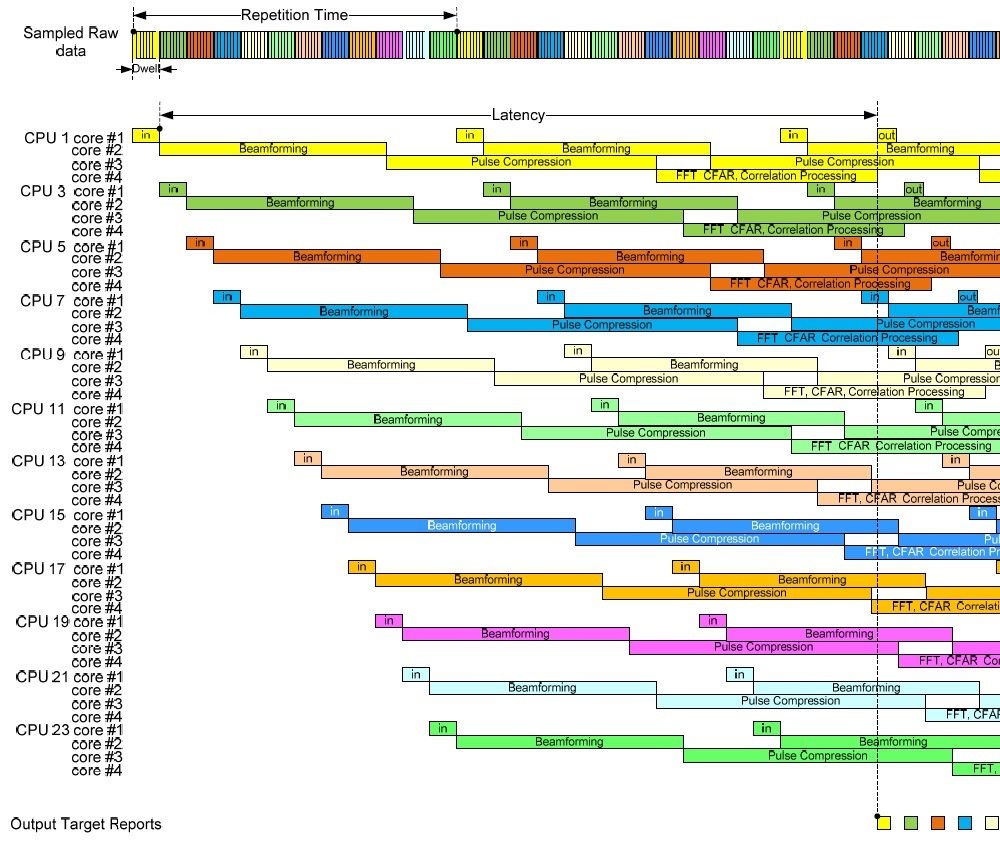
\includegraphics[width=140mm]{figures/aa_scheme1}
	\caption{A/A Mode Processing}
	\label{fig:existing_analysis:aa_scheme1}
\end{figure}


%%%%%%%%%%%%%%%%%%%%%%%%%
%%%%%  SSUB-SECTION   %%%
%%%%%%%%%%%%%%%%%%%%%%%%%
\subsubsection{Scheduling Scheme}
\label{sss:scheme1:aa:sched_blocks}
Scheduling functional blocks in the IMA processor architecture is shown in Figure \ref{fig:existing_analysis:aa_scheme1}. As discussed earlier, only odd numbered CPUs (CPU1,3,5...23) take part in processing A/A Mode algorithm.\\[0.3cm]
\textsl{Core\#1} receives incoming data from the Ethernet and stores them into Core\#1's buffer memory in SDRAM. Then the data is copied to Core\#2's buffer memory.\\[0.2cm]
%%%%%%
\textsl{Core\#2} transfers the data from its buffer memory to storage memory to L2 cache and then performs Beamforming. The results of the processing are stored back to the core\#3's buffer memory in SDRAM.\\[0.2cm]
%%%%%
\textsl{Core\#3} reads the data from its SDRAM partition and performs Pulse Compression. The results of the processing are stored back to the SDRAM.\\[0.2cm]
%%%%%%
\textsl{Core\#4} gets the data from its SDRAM partition and performs FFT, CFAR, Correlation Processing. The results of the processing are stored back to the SDRAM.

%%%%%%%%%%%%%%%%%%%%%%%%%
%%%%%  SSUB-SECTION   %%%
%%%%%%%%%%%%%%%%%%%%%%%%%
\subsubsection{CPU Utilization}
\label{sss:scheme1:aa:cpu_util}
CPU utilization is the ratio of processing time to the available time. The worst case available time of a CPU is the time span between receiving two shortest Dwells by the CPU, calculated as 12x shortest Dwell time. The results reported here are rounded to two decimal places. The burst configurations and processor parameters are stated in the Chapter \ref{ss:aa_mode:radar_char}. Calculations for the first burst of the look direction-1 is explained in Appendix \ref{app:ba:calc:scheme1}. 

%9.83%	11.68%	13.83%	16.32%	19.16%
\begin{figure}
\begin{minipage}{\linewidth}
	\begin{minipage}{0.45\linewidth}
		\resizebox {7cm} {!} {
			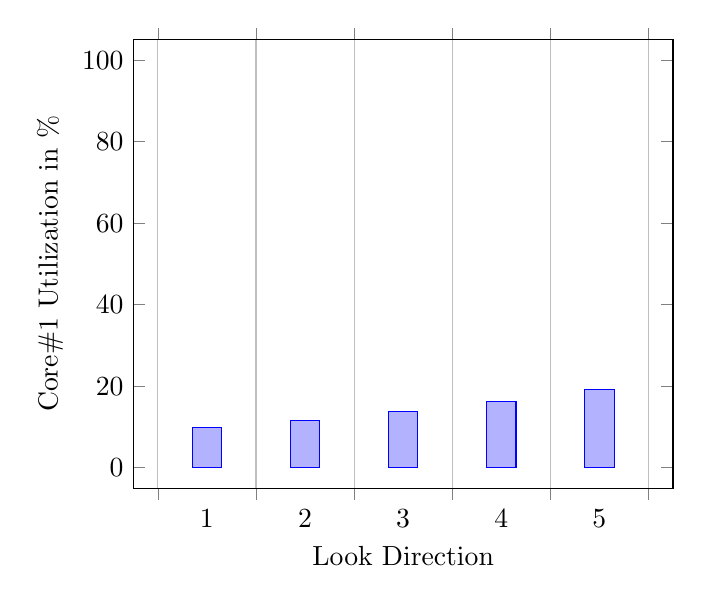
\begin{tikzpicture}{width=7cm}
			\begin{axis}[
				x tick label style={/pgf/number format/1000 sep=},
				ylabel=Core\#1 Utilization in \%,
				xlabel=Look Direction,
				enlargelimits=0.05,
				legend style={at={(0.5,-0.1)},
				anchor=north,legend columns=-1},
				ybar interval=0.3,
				ymin=0,ymax=100,
				]
			\addplot 
				coordinates {(1, 9.83) (2, 11.68) (3, 13.83) (4, 16.32) (5, 19.16) (6, 19.16)};
			\end{axis}
			\end{tikzpicture}
		}
      \end{minipage}
      \hspace{0.05\linewidth}
      \begin{minipage}{0.45\linewidth}
	 \resizebox {7cm} {!} {
		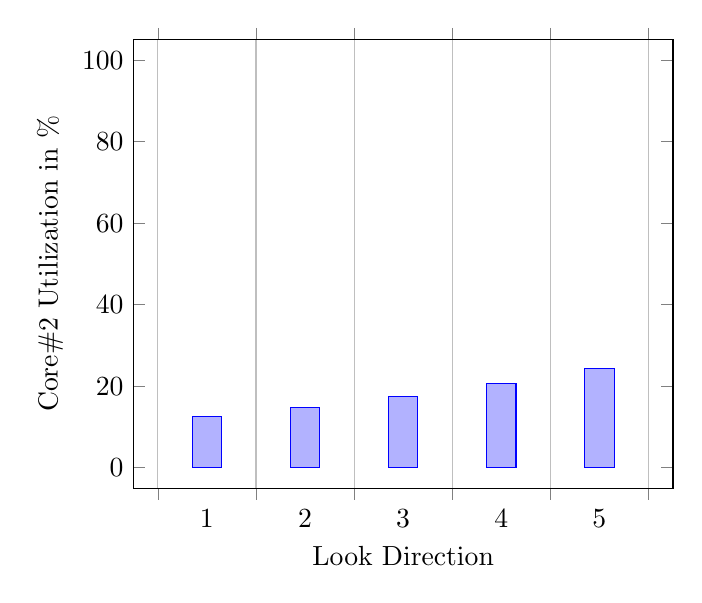
\begin{tikzpicture}{width=5cm}
		\begin{axis}[
			x tick label style={/pgf/number format/1000 sep=},
			ylabel=Core\#2 Utilization in \%,
			xlabel=Look Direction,
			enlargelimits=0.05,
			legend style={at={(0.5,-0.1)},
			anchor=north,legend columns=-1},
			ybar interval=0.3,
			ymin=0,ymax=100,
			]
		\addplot
			coordinates {(1, 12.48) (2, 14.82) (3, 17.56) (4, 20.7) (5, 24.32) (6, 19.16)};
		\end{axis}
		\end{tikzpicture}
		}
	\end{minipage}
\end{minipage}

\vspace*{2cm}
\begin{minipage}{\linewidth}
	\begin{minipage}{0.45\linewidth}
		\resizebox {7cm} {!} {
			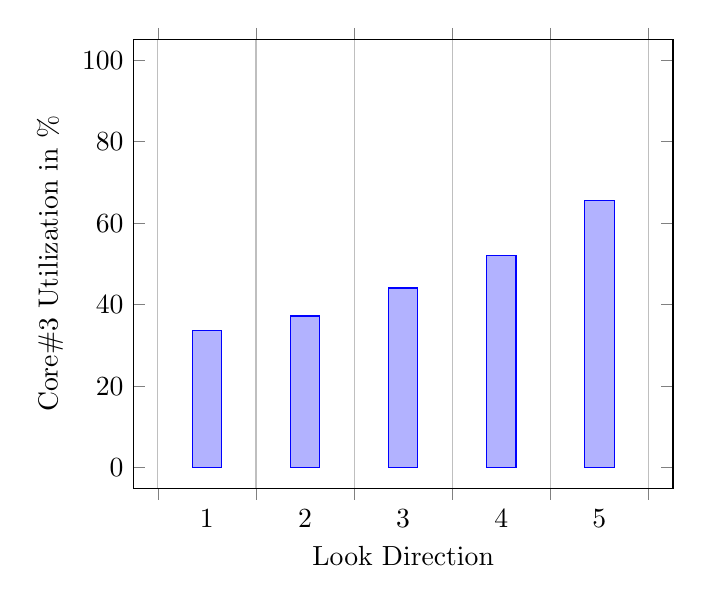
\begin{tikzpicture}{width=7cm}
			\begin{axis}[
				x tick label style={/pgf/number format/1000 sep=},
				ylabel=Core\#3 Utilization in \%,
				xlabel=Look Direction,
				enlargelimits=0.05,
				legend style={at={(0.5,-0.1)},
				anchor=north,legend columns=-1},
				ybar interval=0.3,
				ymin=0,ymax=100,
				]
			\addplot
				coordinates {(1, 33.68) (2, 37.22) (3, 44.1) (4, 52.02) (5, 65.65) (6, 19.16)};
			\end{axis}
			\end{tikzpicture}
		}
      \end{minipage}
      \hspace{0.05\linewidth}
      \begin{minipage}{0.45\linewidth}
	 \resizebox {7cm} {!} {
		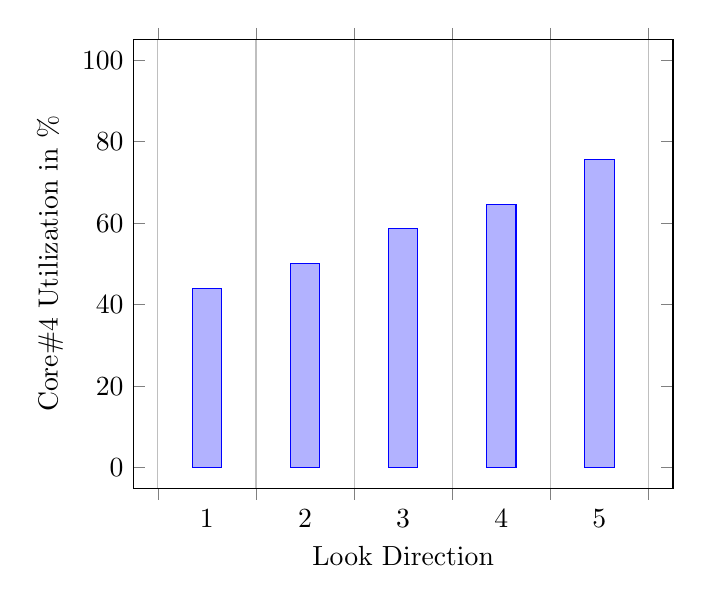
\begin{tikzpicture}{width=5cm}
		\begin{axis}[
			x tick label style={/pgf/number format/1000 sep=},
			ylabel=Core\#4 Utilization in \%,
			xlabel=Look Direction,
			enlargelimits=0.05,
			legend style={at={(0.5,-0.1)},
			anchor=north,legend columns=-1},
			ybar interval=0.3,
			ymin=0,ymax=100,
			]
		\addplot
			coordinates {(1, 43.9) (2, 50.21) (3, 58.67) (4, 64.53) (5, 75.58) (6, 19.16)};
		\end{axis}
		\end{tikzpicture}
		}
	\end{minipage}
\end{minipage}
\caption{CPU Utilization}
\label{ext_ana:sch1:cpu_util}
\end{figure}

CPU utilization is shown in Figure \ref{ext_ana:sch1:cpu_util} for each Core. On every Core, Look Direction-5 contributes to the highest(worst-case) processing time. It is evident from the figure that the Core\#1 and Core\#2 are utilized less than 25\%, meaning that the I/O processing and Beam-forming are not computation intensive. On the other hand, Core\#3 and Core\#4 are utilized 65\% and 75\% of the available time, meaning that there is very less room to adapt future growth. Core\#3 and Core\#4 violates the Radar processor requirements in terms of CPU utilization.

%%%%%%%%%%%%%%%%%%%%%%%%%
%%%%%  SSUB-SECTION   %%%
%%%%%%%%%%%%%%%%%%%%%%%%%
\subsubsection{Processing Latency}
\label{sss:scheme1:latency}
Processing Latency is the time between reception of a Dwell and sending of processed result data. As listed in Table \ref{tbl:existing_analysis:aa_scheme1_latency}, processing latency between 333ms and 617ms is achieved depending on the Look Direction.  Derivation of Look Direction-1's processing latency is explained in Appendix \ref{app:sch1:proc_late}. Number of Dwells the Radar can transmit, while the processor is busy in performing computations of a first received Dwell, is given as \textsl{\#Dwells transmitted}. Higher the \textsl{\#Dwells transmitted} implies that higher the stagnation of received echoes, which decreases the Radar processors response time. According to the Radar processor requirements, \textsl{\#Dwells transmitted} should be less than 2.

Time required to process a complete Dwell relate to the look direction-1 is shown in Figure \ref{fig:mm:scheme1_latency_tot}.
\begin{figure}[h!]
	\centering
	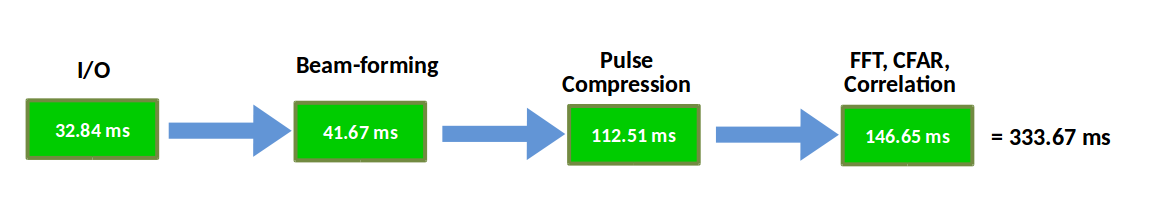
\includegraphics[width=145mm]{figures/scheme1_latency_tot}
	\caption{Dwell Processing time of Look Direction-1}
	\label{fig:mm:scheme1_latency_tot}
\end{figure}


\begin{table}[h!]
	\centering
	\begin{tabular}{|c|l|l|l|} 
	 \hline
	 \textbf{Look direction} & \textbf{Dwell time[ms]} & \textbf{Latency[ms]} & \textbf{\#Dwells transmitted} \\
	 \hline
	 1 & 27.84 & 333.67 & 11.99 \\ \hline
	 2 & 33.07 & 380.61 & 11.51 \\ \hline
	 3 & 39.17 & 448.16 & 11.44 \\ \hline
	 4 & 46.20 & 513.00 & 11.10 \\ \hline
	 5 & 54.26 & 617.05 & 11.37 \\ \hline
	\end{tabular}
	\caption{A/A Mode Processing Latency}
	\label{tbl:existing_analysis:aa_scheme1_latency}
\end{table}

%%%%%%%%%%%%%%%%%%%%%%%%%
%%%%%  SSUB-SECTION   %%%
%%%%%%%%%%%%%%%%%%%%%%%%%
\subsubsection{Memory Utilization}
\label{sec:scheme1:mem_util}
Each CPU has 4GiB of externally connected SDRAM. It is assumed that 3GiB are allocated for OS, storing executable code, etc. 1GiB are available for the actual data processing. Input and output data size for the cores and calculation of the memory requirement are shown Appendix \ref{app:sch1:mem_util}. According to the estimation, 7\% of the available capacity is sufficient for A/A Mode processing.

%%%%%%%%%%%%%%%%%%%%%%%%%
%%%%%  SSUB-SECTION   %%%
%%%%%%%%%%%%%%%%%%%%%%%%%
\subsubsection{Interface Utilization}
\label{sec:scheme1:aa_interface_util}
Interfaces are the data routing paths in the Radar processor. Nominal bandwidth of 100MiB/s data rate is assumed for the interfaces.  Peak interface utilization is calculated as 72\% of the available 100MiB/s. The calculations are listed in Appendix \ref{fig:existing_analysis:aa_scheme1_interface_util}.

\subsubsection{Summary}
The CPUs in the DGPM are physically separated for A/A Mode and A/G Mode; accordingly the results will not change if the Radar processor is performing both the modes simultaneously. Space partitioning has 12x Dwell latency, utilizing 7\% of the available memory, 72\% of the interface and the following CPU utilization factors. Scheme-1 scheduling technique violates the requirements of the Radar processor in terms of processing latency, hence it is not applicable for real-time processing.

\begin{table}[h!]
	\centering
	\begin{tabular}{|l|l|l|l|l|} 
	 \hline
	& \textbf{Core\#1} & \textbf{Core\#2} & \textbf{Core\#3} & \textbf{Core\#4} \\ \hline
	\textbf{Utilization} & 19.16\% & 24.32\% & 65.65\% & 75.58\% \\ \hline
	\end{tabular}
	\caption{CPU Utilization}
\end{table}

\clearpage
%%%%%%%%%%%%%%%%%%%%%%%%%%%%%%%%%%%%%
%%%%%%%%%%%%%%%%%%%%%%%%%%%%%%%%%%%%%
%%%%%%%%%%%%   SECTION   %%%%%%%%%%%%
%%%%%%%%%%%%%%%%%%%%%%%%%%%%%%%%%%%%%
%%%%%%%%%%%%%%%%%%%%%%%%%%%%%%%%%%%%%
\section{Scheme 2 - Time Partitioning}
\label{sec:scheme2}
Every CPU in the IMA processor architecture runs both the A/A mode and A/G mode application concurrently. CPU time and resources are shared for both the applications. Memory is partitioned for each mode to provide segregation. This analysis assumes
\begin{compactitem}
	\item All the four cores of a CPU can access SDRAM without interfering each other.
	\item L2 cache is statically partitioned at compile time, partition values are stated in Figure \ref{fig:existing_analysis:scheme2_partition_values}.
	\item Partition change time is 0.5ms. 
\end{compactitem} 

Figure \ref{fig:existing_analysis:scheme2_partition} shows the time partitioning of a CPU. Each application has to complete processing and suspend itself before the time slice expires. Otherwise a "deadline miss exception" is triggered.

\begin{figure}[h!]
	\centering
	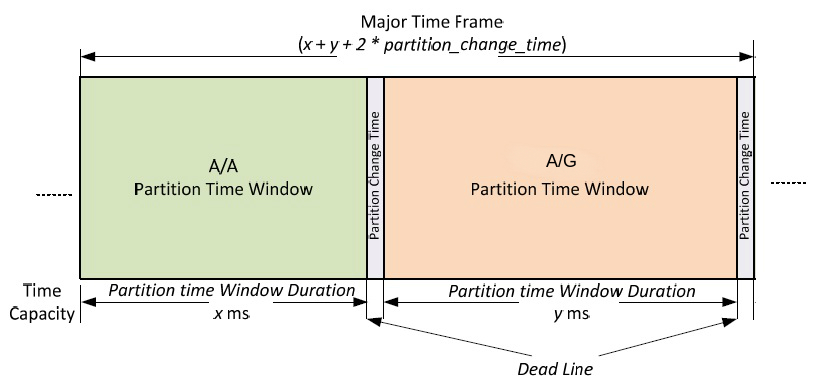
\includegraphics[height=55mm]{figures/scheme2_partition}
	\caption{Time Partition}
	\label{fig:existing_analysis:scheme2_partition}
\end{figure}

A/A data and A/G data are distributed by iCON1 to PSM1 and PSM2 respectively. Processed A/A data are transferred to iCON2 through PSM1. Partially processed A/G results from CPU1...CPU20 are transfered to CPU21...CPU24, where final A/G processing is carried out, followed by the results of the A/G processing are sent via PSM2 and iCON2 to a display.

\begin{figure}[h!]
	\centering
	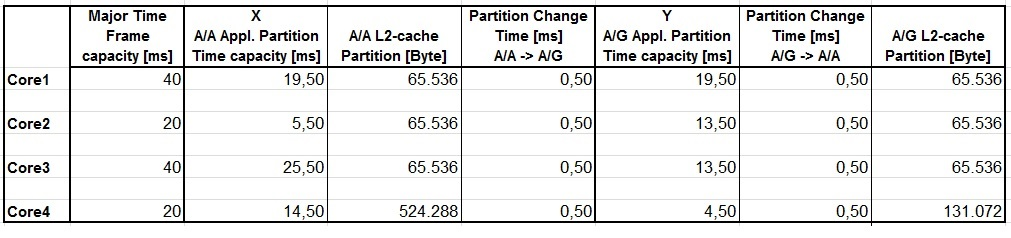
\includegraphics[width=150mm]{figures/scheme2_partition_values}
	\caption{Values for Time Partition}
	\label{fig:existing_analysis:scheme2_partition_values}
\end{figure}

\begin{figure}[h!]
	\centering
	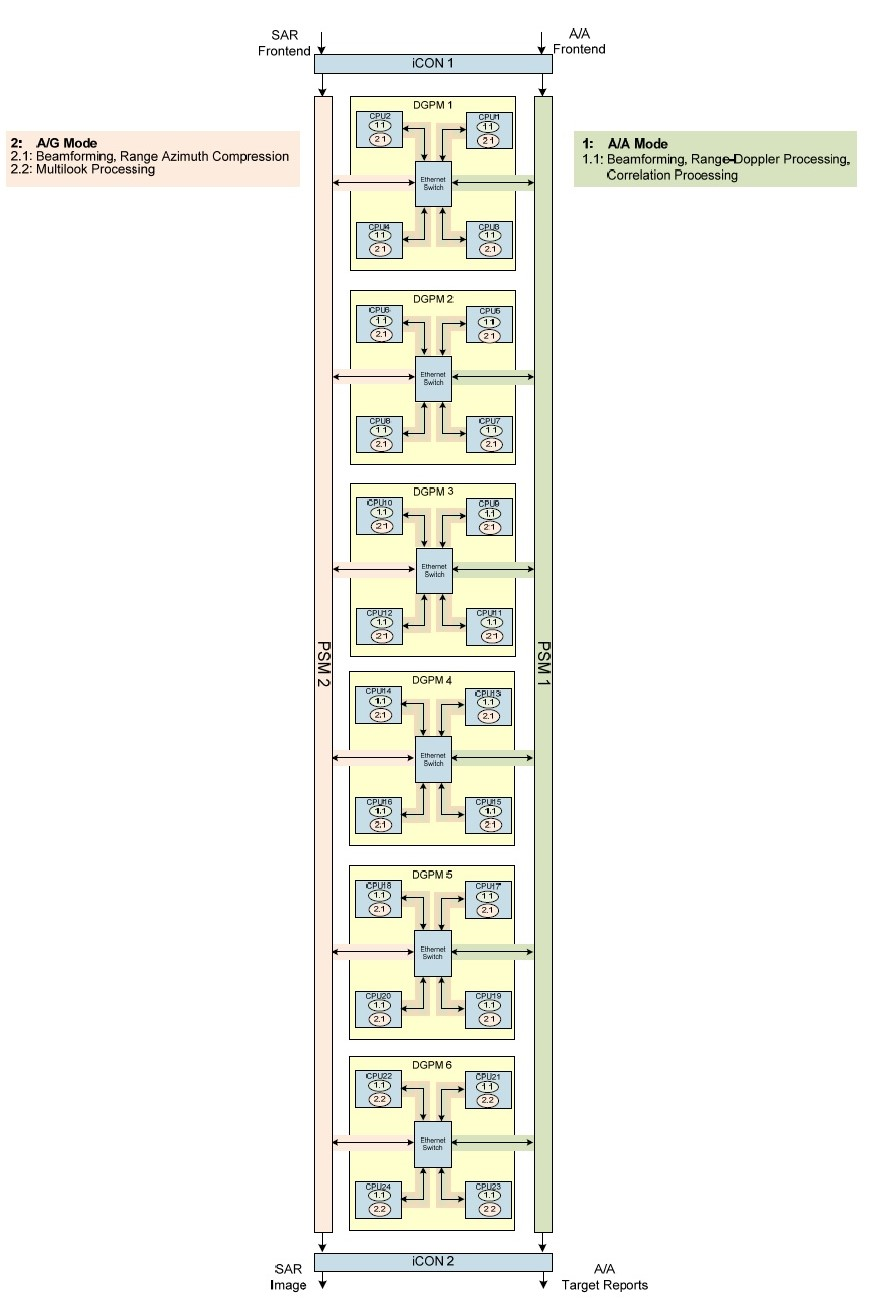
\includegraphics[width=160mm, height=220mm]{figures/scheme2_mode_mapping}
	\caption{Scheduling Scheme}
	\label{fig:existing_analysis:scheme2_mode_mapping}
\end{figure}
\clearpage

\subsection{A/A Mode Results}
\label{ss:scheme2:aa}
A/A Mode configuration is similar to the configuration discussed in Scheme-1, (see Chapter \ref{ss:scheme1:aa}) except that the data is distributed to 24 CPUs. There may be some additional time slots required to fit the processing into the allotted time slice. For instance, 33 time slots would provide sufficient time to complete a certain processing having 65536 loop counts. Therefore 1985 loops could be processed in each time slot. An additional 34$^{th}$ time slot would be required to execute the remaining 31 loops. This is called Time Slot Adjustment. Calculations are same as Scheme-1 and hence details of the cores processing time are not shown for simplicity.

\subsubsection{CPU Utilization}
\label{sss:scheme2:cpu_util}
Available time is 24x shortest Dwell time. Since the core is time sliced, effective available time is reduced by the factor of time slice and the processing latency is increased by the same factor. Table \ref{tbl:existing_analysis:aa_scheme2_cpu_util} lists the peak utilization values of each core.

\begin{table}[h!]
	\centering
	\begin{tabular}{|l|l|l|l|l|} 
	 \hline
	 & \textbf{Core\#1} & \textbf{Core\#2} & \textbf{Core\#3} & \textbf{Core\#4} \\ \hline
	 \textbf{Core Utilization} & 25\% & 53\% & 71\% & 63\% \\ \hline
	\end{tabular}
	\caption{CPU Utilization}
	\label{tbl:existing_analysis:aa_scheme2_cpu_util}
\end{table}

\subsubsection{Processing Latency}
\label{sss:scheme2:latency}
Processing latency is higher than Scheme-1, because a core gets approximately half of the available time for A/A Mode processing. Processing latency between 640ms and 1100ms is achieved depending on the look direction, which is also listed in Table \ref{tbl:existing_analysis:aa_scheme2_latency}.

Time required to process a complete Dwell relate to the look direction-1 is shown in Figure \ref{fig:mm:scheme2_latency_tot}.
\begin{figure}[h!]
	\centering
	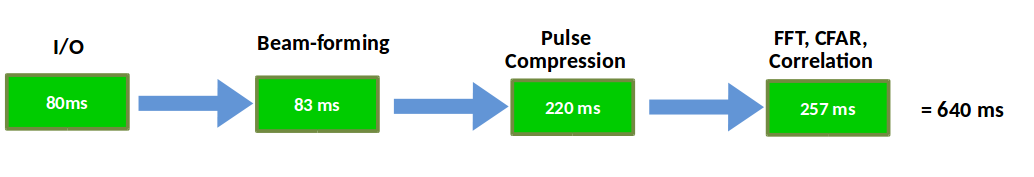
\includegraphics[width=145mm]{figures/scheme2_latency_tot}
	\caption{Dwell Processing time of Look Direction-1}
	\label{fig:mm:scheme2_latency_tot}
\end{figure}

\begin{table}[h!]
	\centering
	\begin{tabular}{|c|l|l|l|} 
	 \hline
	 \textbf{Look direction} & \textbf{Dwell time[ms]} & \textbf{Latency[ms]} & \textbf{\#Dwells transmitted} \\
	 \hline
	 1 & 27.84 & 640 & 22.99 \\ \hline
	 2 & 33.07 & 700 & 21.17 \\ \hline
	 3 & 39.17 & 820 & 20.93 \\ \hline
	 4 & 46.20 & 880.00 & 19.05 \\ \hline
	 5 & 54.26 & 1100 & 20.27 \\ \hline
	\end{tabular}
	\caption{A/A Mode Processing Latency}
	\label{tbl:existing_analysis:aa_scheme2_latency}
\end{table}
\FloatBarrier

\subsubsection{Memory Utilization}
\label{sss:scheme2:mem_util}
Each CPU has 4GiB of externally connected SDRAM. It is assumed that 3GiB are allocated for OS, storing executable code, etc, 1GiB are available for data processing. The peak memory utilization is calculated as 9\% of the available memory.

\subsubsection{Interface Utilization}
\label{sss:scheme2:interface_util}
Data distribution scheme is the extended version of Scheme-1, hence the peak interface utilization remains same as 72\%.

\subsection{Summary}
\label{sss:scheme2:sar_summary}
The Time Partition configuration has 23x Dwell time latency, utilizing 63\% of the CPU, 9\% of the memory and 72\% of the interface capability. Scheme-2 also failed to fulfil the Radar processor requirement. Neither of the baseline analysis scheme satisfies the real-time requirements. A Radar processor, having 23x Dwell time processing latency is not a good choice for airborne Radar processor. Next chapters explain optimal scheduling schemes to bring down the processing latency to an acceptable level.


